\documentclass[tikz,border=2pt]{standalone}
\usepackage{amsmath,amssymb}
\usepackage{tikz}
\usetikzlibrary{arrows.meta}

\begin{document}
% Three stationary points (grad f = 0) seen through their level sets: closed loops around a
% peak (Hessian negative definite: local max), around a pit (positive definite: local min),
% crossing curves at a saddle (indefinite).
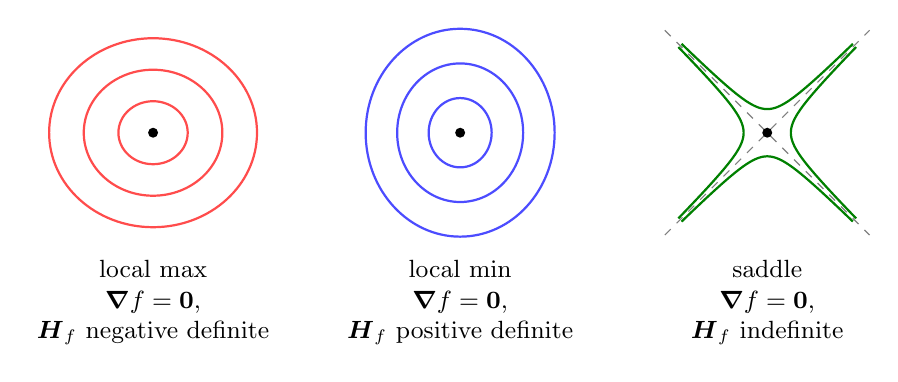
\begin{tikzpicture}[every node/.style={font=\small}]
	\begin{scope}
		\foreach \r in {0.4,0.8,1.2} {\draw[red!70, thick] (0,0) ellipse ({\r*1.1} and {\r});}
		\fill (0,0) circle (1.8pt);
		\node[anchor=north, align=center] at (0,-1.5) {local max\\ $\boldsymbol{\nabla} f=\boldsymbol{0}$,\\ $\boldsymbol{H}_f$ negative definite};
	\end{scope}
	\begin{scope}[xshift=3.9cm]
		\foreach \r in {0.4,0.8,1.2} {\draw[blue!70, thick] (0,0) ellipse ({\r} and {\r*1.1});}
		\fill (0,0) circle (1.8pt);
		\node[anchor=north, align=center] at (0,-1.5) {local min\\ $\boldsymbol{\nabla} f=\boldsymbol{0}$,\\ $\boldsymbol{H}_f$ positive definite};
	\end{scope}
	\begin{scope}[xshift=7.8cm]
		% Exact saddle model q=x_1^2-x_2^2: green curves q=+/-0.09.
        \def\levscale{0.3}
        \foreach \sgn in {-1,1} {
            \draw[green!50!black,thick] plot[domain=-2:2,samples=80,variable=\t] ({\sgn*\levscale*cosh(\t)},{\levscale*sinh(\t)});
            \draw[green!50!black,thick] plot[domain=-2:2,samples=80,variable=\t] ({\levscale*sinh(\t)},{\sgn*\levscale*cosh(\t)});
        }
		\draw[gray, dashed] (-1.3,-1.3) -- (1.3,1.3);
		\draw[gray, dashed] (-1.3,1.3) -- (1.3,-1.3);
		\fill (0,0) circle (1.8pt);
		\node[anchor=north, align=center] at (0,-1.5) {saddle\\ $\boldsymbol{\nabla} f=\boldsymbol{0}$,\\ $\boldsymbol{H}_f$ indefinite};
	\end{scope}
\end{tikzpicture}
\end{document}
